\documentclass[tikz,border=2pt]{standalone}
\usepackage{amsmath}
\usetikzlibrary{arrows.meta,positioning,fit,backgrounds}
\begin{document}
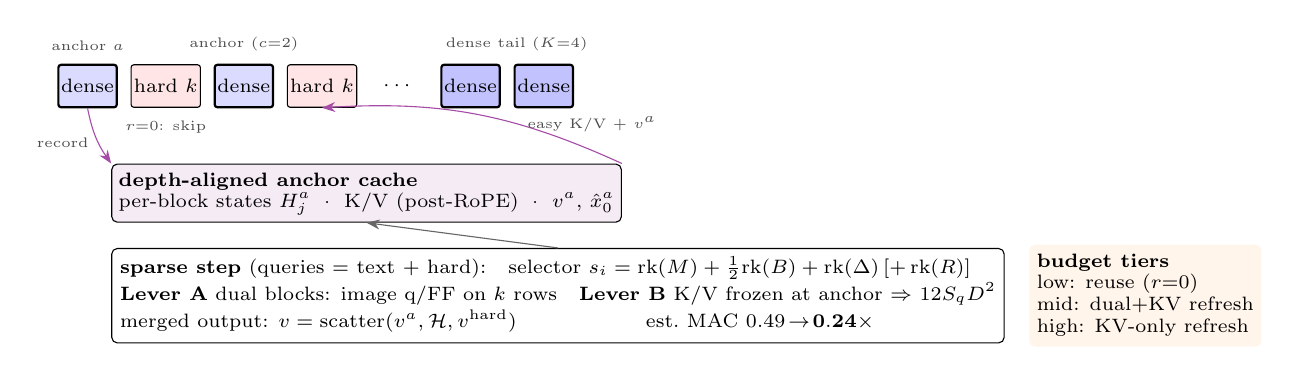
\begin{tikzpicture}[
  font=\scriptsize, >=Stealth,
  stp/.style={draw, rounded corners=1pt, minimum width=7.2mm, minimum height=5.4mm, inner sep=1pt},
  anch/.style={stp, fill=blue!14, thick},
  sprs/.style={stp, fill=red!10},
  tl/.style={stp, fill=blue!24, thick},
  lbl/.style={font=\tiny, text=black!70},
  cachebox/.style={draw, rounded corners=2pt, fill=violet!8, minimum height=5.4mm, inner sep=2.5pt},
]
% ---------------- timeline ----------------
\node[anch] (s0) {dense};
\node[sprs, right=1.6mm of s0] (s1) {hard $k$};
\node[anch, right=1.6mm of s1] (s2) {dense};
\node[sprs, right=1.6mm of s2] (s3) {hard $k$};
\node[stp, right=1.6mm of s3, draw=none] (dots) {$\cdots$};
\node[tl, right=1.6mm of dots] (t1) {dense};
\node[tl, right=1.6mm of t1] (t2) {dense};

\node[lbl, above=0.4mm of s0] {anchor $a$};
\node[lbl, above=0.4mm of s2] {anchor ($c{=}2$)};
\node[lbl, above=0.4mm of t1.north east, xshift=2mm] {dense tail ($K{=}4$)};
\node[lbl, below=0.4mm of s1] {$r{=}0$: skip};

% ---------------- cache ----------------
\node[cachebox, below=7mm of s2.south west, anchor=north west, xshift=-13mm]
  (cache) {\begin{tabular}{@{}l@{}}
    \textbf{depth-aligned anchor cache}\\[-0.2mm]
    per-block states $H_j^{a}$ \;·\; K/V (post-RoPE) \;·\; $v^{a}$, $\hat{x}_0^{a}$
  \end{tabular}};
\draw[->, violet!70] (s0.south) to[bend right=12] node[lbl, left, pos=.6]{record} (cache.north west);
\draw[->, violet!70] (cache.north east) to[bend right=14]
  node[lbl, right, pos=.35]{easy K/V + $v^{a}$} (s3.south);

% ---------------- sparse step detail ----------------
\node[draw, rounded corners=2pt, below=3.2mm of cache.south west, anchor=north west, inner sep=3pt]
  (detail) {\begin{tabular}{@{}l@{}}
  \textbf{sparse step} (queries $=$ text $+$ hard):\quad
  selector $s_i=\mathrm{rk}(M)+\tfrac12\mathrm{rk}(B)+\mathrm{rk}(\Delta)\,[+\,\mathrm{rk}(R)]$\\[0.4mm]
  \textbf{Lever A} dual blocks: image q/FF on $k$ rows\quad
  \textbf{Lever B} K/V frozen at anchor $\Rightarrow$ $12S_qD^2$\\[0.4mm]
  merged output: $v=\mathrm{scatter}(v^{a},\mathcal{H},v^{\mathrm{hard}})$
  \hfill est.\ MAC $0.49\!\to\!\mathbf{0.24}\times$
  \end{tabular}};
\draw[->, black!60] (detail.north) -- (cache.south);

% ---------------- tiers ----------------
\node[draw=none, right=4mm of detail.east, anchor=west, inner sep=0] (tiers)
  {\begin{tabular}{@{}l@{}}
   \textbf{budget tiers}\\[-0.2mm]
   low: reuse ($r{=}0$)\\
   mid: dual$+$KV refresh\\
   high: KV-only refresh
  \end{tabular}};
\begin{scope}[on background layer]
\node[fit=(tiers), fill=orange!8, rounded corners=2pt, inner sep=2.5pt] {};
\end{scope}
\end{tikzpicture}
\end{document}
